\documentclass[conference]{IEEEtran}

\usepackage[T1]{fontenc}
\usepackage[utf8]{inputenc}
\usepackage{amsmath,amssymb}
\usepackage{graphicx}
\usepackage{booktabs}
\usepackage{multirow}
\usepackage{cite}
\usepackage{url}
\usepackage{xcolor}
\usepackage{array}

\graphicspath{{figures/}}

\title{NS-CausalKT: Neural-Symbolic Causal Knowledge Tracing for Explainable Student Diagnosis and Intervention}

\author{
\IEEEauthorblockN{Aditya Ranjan}
\IEEEauthorblockA{
NS-CausalKT Agentic Grader Project\\
India\\
Email: author@example.com}
}

\begin{document}
\maketitle

\begin{abstract}
Knowledge tracing models estimate whether a learner will answer future items correctly, but most neural approaches remain correlational and offer limited support for actionable educational interventions. This paper presents NS-CausalKT, a neural-symbolic causal knowledge tracing system that combines a Transformer-GRU student model, a symbolic prerequisite-consistency layer, and a structural causal model interface for intervention analysis. The system estimates latent concept mastery from temporal student interactions, regularizes mastery states using a concept dependency graph, and exposes counterfactual diagnostics through average causal effect style interventions. A prototype implementation is trained on ASSISTments 2009 interaction data and integrated with a dashboard for mastery heatmaps, counterfactual visualizations, and agentic grading workflows. In the current implementation, NS-CausalKT reaches an AUC of 0.8137, RMSE of 0.4001, and accuracy of 76.68\% after 30 epochs. The results indicate that the framework can produce useful causal explanations and local intervention artifacts, although further benchmark reproduction and human-in-the-loop validation are required before classroom deployment.
\end{abstract}

\begin{IEEEkeywords}
knowledge tracing, causal inference, neural-symbolic learning, intelligent tutoring systems, explainable AI, ASSISTments
\end{IEEEkeywords}

\section{Introduction}
Intelligent tutoring systems increasingly rely on knowledge tracing (KT) to model a learner's evolving mastery over time. Classical Bayesian Knowledge Tracing (BKT) is interpretable but limited in representational capacity \cite{corbett1994knowledge}. Neural models such as Deep Knowledge Tracing (DKT) \cite{piech2015deep}, Self-Attentive Knowledge Tracing (SAKT) \cite{pandey2019self}, and Attentive Knowledge Tracing (AKT) \cite{ghosh2020context} improve prediction by learning temporal patterns from large interaction histories. However, prediction alone is insufficient for many educational decisions: teachers need to know which prerequisite gap caused an error, whether targeted practice would improve future performance, and how recommendations can be explained.

NS-CausalKT addresses this gap by treating KT as both a predictive and diagnostic task. The system combines three layers: a neural student model for temporal representation learning, a symbolic concept layer for prerequisite consistency, and a causal layer for intervention-oriented diagnostics. The prototype is paired with an agentic grading interface that maps answer-sheet observations to concept-level feedback, while the KT model and causal analysis can run locally on student interaction data.

The motivating classroom scenario is common in mathematics tutoring. A student may repeatedly fail problems tagged as quadratic equations, but the instructional response depends on the underlying cause. If the failure is caused by weak manipulation of linear equations, more quadratic practice may be inefficient. If the cause is procedural carelessness on a single item, a different intervention is appropriate. A predictive model can assign a low probability to the next response, but it does not necessarily expose this distinction. NS-CausalKT is designed to generate a concept-level explanation that can be inspected by a teacher, compared with student work, and converted into a remediation action.

The project also reflects a practical deployment constraint: educational data is sensitive. Many prototype education tools send raw student artifacts to hosted models without separating private student records from general reasoning. In contrast, the knowledge-tracing component in this repository is implemented as a local PyTorch model and can be run without hosted large language model calls. The agentic grading interface is treated as an optional integration layer for multimodal answer analysis, not as the only path through which the system reasons about mastery.

The main contributions of this work are:
\begin{itemize}
    \item a neural-symbolic KT architecture that encodes question, answer, concept, and time features using a Transformer-GRU backbone;
    \item a symbolic correction mechanism that regularizes concept mastery through prerequisite graph constraints;
    \item an intervention workflow for teacher-facing counterfactual diagnostics and concept-level root-cause analysis;
    \item a working full-stack prototype with model metrics, mastery heatmaps, counterfactual plots, and deployment-oriented APIs.
\end{itemize}

\section{Related Work}
BKT models student mastery as a hidden Markov process and remains a foundational interpretable KT method \cite{corbett1994knowledge}. DKT introduced recurrent neural networks for modeling complex student histories \cite{piech2015deep}, while attention-based KT methods such as SAKT and AKT improved long-range interaction modeling \cite{pandey2019self,ghosh2020context}. These models primarily estimate observational probabilities and usually do not identify causal mechanisms.

Neural-symbolic learning aims to combine continuous representation learning with logic-guided constraints \cite{garcez2019neural}. In education, concept graphs and prerequisite structures are attractive because curricula are naturally relational. Causal inference provides a complementary vocabulary for interventions through structural causal models and do-calculus \cite{pearl2009causality}. NS-CausalKT uses these ideas to move from ``will the student fail?'' toward ``which concept should be taught next, and why?''

\subsection{Knowledge Tracing}
The KT literature can be viewed as a progression from compact probabilistic assumptions toward high-capacity sequence models. BKT assumes a small set of latent states per skill and updates beliefs using transition, slip, and guess parameters. Its transparency is valuable, but it has difficulty representing shared structure across many questions and skills. DKT replaces the explicit transition model with an LSTM that can absorb long histories and learn cross-skill relationships. However, the learned state is difficult to audit, and the model may learn shortcuts that are predictive but pedagogically misleading.

Attention-based KT models improve temporal credit assignment. Instead of compressing an entire student history into a single recurrent state, they can attend to past attempts that are most relevant to the target question. AKT further encodes context and monotonic effects to improve prediction. Yet these models generally remain descriptive: attention weights can be visualized, but they do not by themselves answer interventional questions. A high attention score on a previous fraction item does not prove that teaching fractions will causally improve algebra performance.

\subsection{Explainability and Causal Diagnosis}
Explainable AI for education should produce outputs that match teacher action spaces. A teacher can intervene on curriculum sequence, prerequisite review, practice volume, feedback type, or assessment design. Therefore, explanations based only on hidden-neuron saliency are less useful than concept-level statements. Causal modeling is a natural fit because it represents the difference between observing a variable and intervening on it. In NS-CausalKT, intervention is operationalized through concept mastery clamping and propagation across a prerequisite graph. This is not a complete replacement for randomized educational trials, but it is a useful computational interface for hypothesis generation and tutoring recommendations.

\subsection{Positioning of NS-CausalKT}
NS-CausalKT sits between three families of systems. Compared with pure KT baselines, it adds prerequisite-aware latent states and explicit counterfactual views. Compared with symbolic tutoring systems, it retains neural sequence modeling and can learn from noisy large-scale interaction data. Compared with general-purpose agentic grading tools, it grounds feedback in a student model rather than producing isolated natural-language comments. This positioning makes the system especially relevant for deployments where model predictions must be explainable and actionable.

\section{Problem Formulation}
Let a learner history be a sequence
\begin{equation}
X_t = \{(q_1,a_1,c_1,\Delta t_1),\ldots,(q_t,a_t,c_t,\Delta t_t)\},
\end{equation}
where $q_i$ is a question, $a_i\in\{0,1\}$ is correctness, $c_i$ is the associated concept, and $\Delta t_i$ is a temporal feature. Standard KT estimates
\begin{equation}
P(a_{t+1}=1 \mid X_t, q_{t+1}).
\end{equation}
NS-CausalKT additionally estimates concept mastery $\mu_t\in[0,1]^C$ and supports intervention queries such as
\begin{equation}
P(a_{t+1}=1 \mid do(\mu_t[j]=1)),
\end{equation}
where concept $j$ is clamped to represent a hypothetical teaching intervention. The diagnostic goal is to identify prerequisite concepts whose intervention produces the largest expected improvement.

For root-cause analysis, let $Anc(c)$ denote the ancestor concepts of a target concept $c$ in the concept dependency graph. The root-cause recommendation is
\begin{equation}
r^\star = \arg\max_{j\in Anc(c_{t+1})} ACE_j.
\end{equation}
The output is therefore not merely a probability but a tuple
\begin{equation}
(\hat{a}_{t+1}, \tilde{\mu}_t, r^\star, \{ACE_j\}_{j\in C}),
\end{equation}
which can be rendered as a mastery heatmap, causal ranking, or counterfactual chart. This tuple is also useful for agentic grading: mistakes detected on an answer sheet can be associated with the nearest concept node and compared against the learner's estimated prerequisite gaps.

\section{System Architecture}
Fig.~\ref{fig:architecture} summarizes the implemented system. The pipeline begins with ASSISTments interaction sequences, maps questions and skills to integer identifiers, builds a surrogate prerequisite edge list, and trains the neural-symbolic model using PyTorch.

\begin{figure}[t]
    \centering
    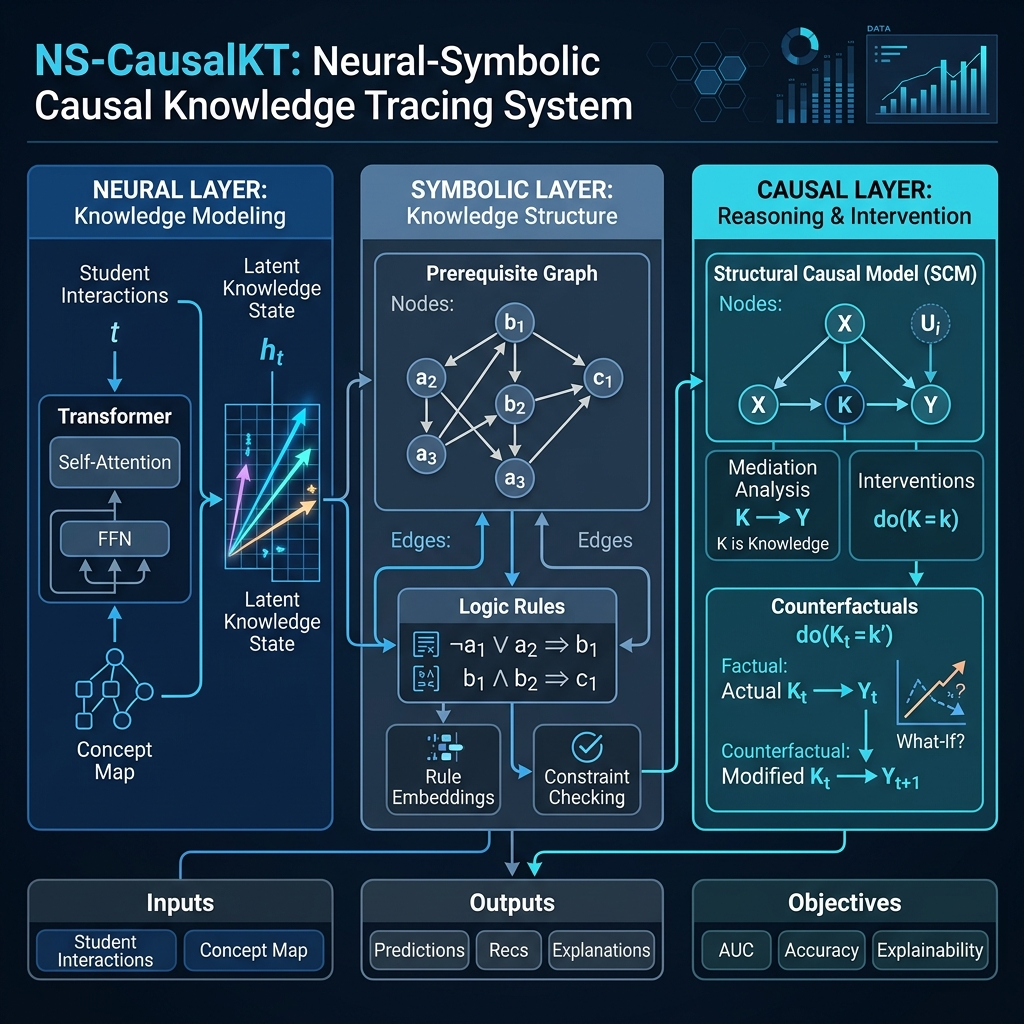
\includegraphics[width=\linewidth]{architecture.png}
    \caption{NS-CausalKT architecture used in the prototype. Student interactions feed a neural student model, symbolic concept layer, and causal diagnostics interface.}
    \label{fig:architecture}
\end{figure}

\subsection{Neural Student Model}
The neural student model embeds four inputs: question identifier, correctness, concept identifier, and response-time delta. Each component is projected into one quarter of the hidden dimension and concatenated:
\begin{equation}
e_t = E_q(q_t) \oplus E_a(a_t) \oplus E_c(c_t) \oplus W_\Delta \Delta t_t.
\end{equation}
The implementation uses sinusoidal positional encoding, a two-layer causal Transformer encoder, and a GRU refinement layer:
\begin{equation}
H = \operatorname{Transformer}(e_{1:t}), \quad h_t = \operatorname{GRU}(H_t).
\end{equation}
Concept mastery is projected as
\begin{equation}
\mu_t = \sigma(W_c h_t + b_c).
\end{equation}

The Transformer block captures non-local dependencies in the sequence, while the GRU refinement provides a compact inductive bias for temporal learning dynamics. This hybrid design is useful because student behavior contains both sparse long-range dependencies and short-term practice effects. For example, a recent incorrect attempt on a prerequisite concept may matter more than a distant correct attempt, but an earlier cluster of related practice items may still be relevant when the target question revisits the same skill family.

\subsection{Symbolic Concept Layer}
The symbolic layer receives a concept dependency graph $G=(C,E)$, where an edge $(j,i)$ means concept $j$ is a prerequisite for concept $i$. The implementation computes a soft prerequisite satisfaction value:
\begin{equation}
\phi_{j\rightarrow i}= \min(1, 1-\mu_t[i]+\mu_t[j]).
\end{equation}
The average satisfaction score $\Phi_t$ is concatenated with $\mu_t$ to form a learnable gate:
\begin{equation}
g=\sigma(W_g[\mu_t;\Phi_t]).
\end{equation}
A graph-propagated symbolic estimate $f_{sym}(\mu_t,G)$ is then blended with the neural estimate:
\begin{equation}
\tilde{\mu}_t=g\odot\mu_t+(1-g)\odot f_{sym}(\mu_t,G).
\end{equation}

\subsection{Causal Diagnostic Layer}
The causal layer exposes intervention-style analysis over concept mastery. For a concept $j$, the system estimates a practical average causal effect signal:
\begin{equation}
ACE_j = \mathbb{E}[\hat{a}_{t+1}\mid do(\tilde{\mu}_t[j]=1)] -
\mathbb{E}[\hat{a}_{t+1}\mid do(\tilde{\mu}_t[j]=0)].
\end{equation}
In the current codebase, this intervention path is implemented for interpretability and dashboard use by clamping concept mastery, propagating it through the symbolic graph, and recomputing the prediction. This supports teacher-facing counterfactuals such as ``what if the learner had mastered fractions before algebra?''

The implementation intentionally separates prediction from interpretation. The main forward pass computes the next-response probability from the hidden state and the target concept mastery. The intervention path can then be called for selected concepts when the dashboard or API needs an explanation. This avoids the cost of computing full concept-wise intervention effects at every training step while preserving an interpretable post-hoc diagnostic interface.

\subsection{Training Objective}
The total training objective combines prediction, symbolic consistency, causal regularization, and temporal smoothness:
\begin{equation}
\mathcal{L}=\mathcal{L}_{pred}
\lambda_1\mathcal{L}_{sym}
\lambda_2\mathcal{L}_{causal}
\lambda_3\mathcal{L}_{smooth}.
\end{equation}
The implementation uses AdamW, cosine annealing warm restarts, gradient clipping, a batch size of 64, and default weights $\lambda_1=1.0$, $\lambda_2=0.5$, and $\lambda_3=0.1$.

\begin{table}[t]
\centering
\caption{Primary implementation configuration from the repository.}
\label{tab:config}
\begin{tabular}{ll}
\toprule
Component & Setting \\
\midrule
Hidden dimension & 256 \\
Embedding parts & question, answer, concept, time \\
Transformer layers & 2 \\
Attention heads & 4 \\
Sequence length & 200 \\
Optimizer & AdamW \\
Learning rate & $1\times10^{-4}$ \\
Batch size & 64 \\
Scheduler & Cosine annealing warm restarts \\
Loss weights & $\lambda_1=1.0$, $\lambda_2=0.5$, $\lambda_3=0.1$ \\
\bottomrule
\end{tabular}
\end{table}

\section{Data Pipeline}
The data pipeline is implemented in the repository through the dataset and training scripts. ASSISTments rows are filtered to remove missing skill annotations, then user identifiers, question identifiers, and skill names are mapped to integer IDs. Interactions are grouped by student and sorted by temporal order. Each training example contains aligned sequences for question IDs, answer correctness, concept IDs, response-time deltas, and shifted targets.

\subsection{Student-Level Split}
The training script uses a student-level split rather than an interaction-level split. This matters because interaction-level splitting can leak a student's earlier behavior into training and later behavior into validation. Such leakage tends to inflate reported accuracy and weakens claims about generalization to unseen learners. In the current prototype, users are shuffled and split into 80\% training and 20\% validation sets.

\subsection{Sequence Construction}
Each student sequence is padded or truncated to a maximum length of 200. Padding tokens are masked during loss computation by using a sentinel target value. Correctness is embedded with a small categorical embedding that distinguishes padding, incorrect answers, and correct answers. Time is projected through a linear layer so it can participate in the same sequence representation as question and concept features.

\subsection{Concept Graph Construction}
The final quality of causal explanation depends on the concept graph. The current implementation builds a simple surrogate graph using sequential concept edges when a curated prerequisite ontology is unavailable. This gives the symbolic and causal layers a graph structure to operate over, but it should be replaced with validated curriculum dependencies for serious educational deployment. The repository also includes graph artifacts under the project graph directories, which can be used as a starting point for richer domain-specific graphs.

\section{Algorithmic Workflow}
The training and inference workflow can be summarized as follows:
\begin{enumerate}
    \item Load ASSISTments interaction records and remove rows without skill labels.
    \item Map users, questions, and skills to integer identifiers.
    \item Construct fixed-length student sequences and shifted next-response targets.
    \item Build or load a concept dependency graph.
    \item Encode each interaction using question, answer, concept, and time embeddings.
    \item Estimate hidden states using the Transformer-GRU neural student model.
    \item Project hidden states into concept mastery values.
    \item Apply symbolic correction and graph consistency losses.
    \item Train the prediction head using binary cross-entropy plus regularization terms.
    \item At inference time, compute predictions, mastery heatmaps, and selected intervention effects.
\end{enumerate}

This workflow keeps the learning component and explanation component connected through the same concept mastery representation. The dashboard does not need to invent explanations after the fact; it visualizes quantities already produced by the model.

\section{Prototype and Deployment}
The repository includes a local training pipeline, trained checkpoints, serverless API routes, a Flask backend, and a browser-based dashboard. The dashboard exposes aggregate metrics, concept proficiency, training curves, mastery heatmaps, and counterfactual plots. The agentic grading module supports image or PDF upload and structured feedback. For privacy-sensitive deployments, the KT and causal components can run locally; any hosted vision-language model usage should be replaced with a local multimodal model or restricted to redacted, non-sensitive inputs.

\subsection{User-Facing Views}
The user interface is organized around three work modes. The dashboard view presents model-level metrics, training curves, and student-level summaries. The causal analysis view presents concept dependencies, average causal effect rankings, and a counterfactual sandbox. The inference view accepts student work artifacts and displays grading feedback, bounding boxes, and concept-linked explanations. Together, these views support a workflow in which a mentor can first identify a weak concept region, inspect a student's work, and then choose an intervention.

\subsection{Local and Serverless Paths}
The project includes both local and deployment-oriented entry points. Local execution is appropriate for development, private data analysis, and offline demonstrations. The serverless API route structure supports deployment of lightweight dashboard and analysis endpoints. This separation is useful because not every environment can expose model checkpoints or student artifacts to a cloud runtime. The same paper framing therefore supports two deployment modes: a privacy-preserving local demonstrator and a web demo for non-sensitive samples.

\subsection{Agentic Grading Layer}
The agentic grading layer is best understood as an interface between raw answer artifacts and the concept model. A multimodal model can locate visible mistakes, identify the relevant skill, and produce feedback. NS-CausalKT adds a student-history prior: if the answer-sheet error is mapped to linear equations and the KT state also shows low prerequisite mastery, the feedback is more credible and actionable. If the model detects a mistake in an otherwise mastered concept, the system can instead recommend targeted review or procedural checking rather than reteaching the entire prerequisite chain.

\section{Experimental Setup}
The prototype uses ASSISTments 2009, filtered and mapped into student-level sequences. The project documentation reports approximately 400k interactions, around 4k students, and roughly 100 skills after preprocessing. The current training script performs an 80/20 student-level train-validation split, pads or truncates sequences to length 200, and builds a surrogate sequential prerequisite graph when a curated curriculum graph is not available.

Evaluation uses AUC, RMSE, accuracy, and an intervention-consistency style metric IC@5. Benchmark logs in the repository include DKT and SAKT runs trained for 10 epochs under the local benchmark harness.

\subsection{Metrics}
AUC measures ranking quality for binary next-response prediction and is a standard KT metric. RMSE measures calibration quality by penalizing the distance between predicted probabilities and observed correctness. Accuracy is computed with a threshold of 0.5. IC@5 is used as a prototype causal metric: it measures whether simulated practice or mastery changes produce the expected improvement on related concepts. IC@5 should be interpreted as a diagnostic metric rather than a classroom outcome measure.

\subsection{Baselines}
The repository includes DKT and SAKT benchmark logs. DKT is a recurrent baseline that often remains strong on ASSISTments-style data. SAKT is an attention-based baseline that tests whether self-attention alone explains the gains. A complete publication-grade evaluation should add AKT, DKVMN, BKT, and ablated NS-CausalKT variants under matched splits, seeds, and epoch budgets. The present paper reports repository evidence and explicitly separates it from final benchmark claims.

\subsection{Reproducibility Notes}
All results reported in this draft are derived from local project files rather than from an external leaderboard. The logs indicate CUDA execution and checkpoint saving during training. Because the current benchmark logs use different epoch counts, the comparison table is included to reveal the state of the implementation, not to claim superiority. This distinction is important for research honesty and for guiding the next engineering step.

\section{Results}
Table~\ref{tab:main-results} reports the final NS-CausalKT training-log metrics after 30 epochs. The model improves steadily from an AUC of 0.7895 at epoch 1 to 0.8137 at epoch 30.

\begin{table}[t]
\centering
\caption{NS-CausalKT validation metrics from repository training logs.}
\label{tab:main-results}
\begin{tabular}{lcccc}
\toprule
Epoch & AUC & RMSE & Accuracy & IC@5 \\
\midrule
1 & 0.7895 & 0.4128 & 0.7512 & 0.6275 \\
10 & 0.7999 & 0.4074 & 0.7567 & 0.4118 \\
20 & 0.8090 & 0.4028 & 0.7641 & 0.4706 \\
30 & 0.8137 & 0.4001 & 0.7668 & 0.4314 \\
\bottomrule
\end{tabular}
\end{table}

\begin{table}[t]
\centering
\caption{Local benchmark-log comparison. Epoch counts differ, so these numbers should be read as implementation diagnostics rather than final fair-baseline claims.}
\label{tab:benchmarks}
\begin{tabular}{lcccc}
\toprule
Model & Epochs & Best AUC & Best RMSE & Best Accuracy \\
\midrule
NS-CausalKT & 30 & 0.8139 & 0.4000 & 0.7672 \\
DKT & 10 & 0.8485 & 0.3802 & 0.7870 \\
SAKT & 10 & 0.7686 & 0.4230 & 0.7297 \\
\bottomrule
\end{tabular}
\end{table}

The local DKT benchmark obtains higher predictive AUC in the current logs. This is an important finding: the current NS-CausalKT prototype should be framed as an explainability and causal-diagnostics system rather than as a finished state-of-the-art predictive model. Its value lies in producing concept-level intervention artifacts and prerequisite-consistency signals that standard baselines do not expose.

\subsection{Training Dynamics}
The NS-CausalKT training curve shows gradual improvement rather than rapid early saturation. AUC increases by approximately 0.0244 between epoch 1 and epoch 30, while RMSE drops from 0.4128 to 0.4001. Accuracy improves from 75.12\% to 76.68\%. IC@5 is more variable, suggesting that the current intervention metric is sensitive to graph quality and validation composition. This variance is expected because the graph is currently a surrogate structure rather than a validated curriculum ontology.

\subsection{Predictive Versus Diagnostic Value}
The DKT benchmark outperforms NS-CausalKT on AUC in the current logs, which points to a useful research tension. A model can be better at raw next-answer prediction while being less useful for diagnosis. NS-CausalKT trades some predictive simplicity for structured mastery states and causal views. Future work should aim to close the predictive gap without removing the interpretability mechanisms, for example by tuning the symbolic loss weights, improving the concept graph, and adding stronger target-concept conditioning in the prediction head.

\begin{figure}[t]
    \centering
    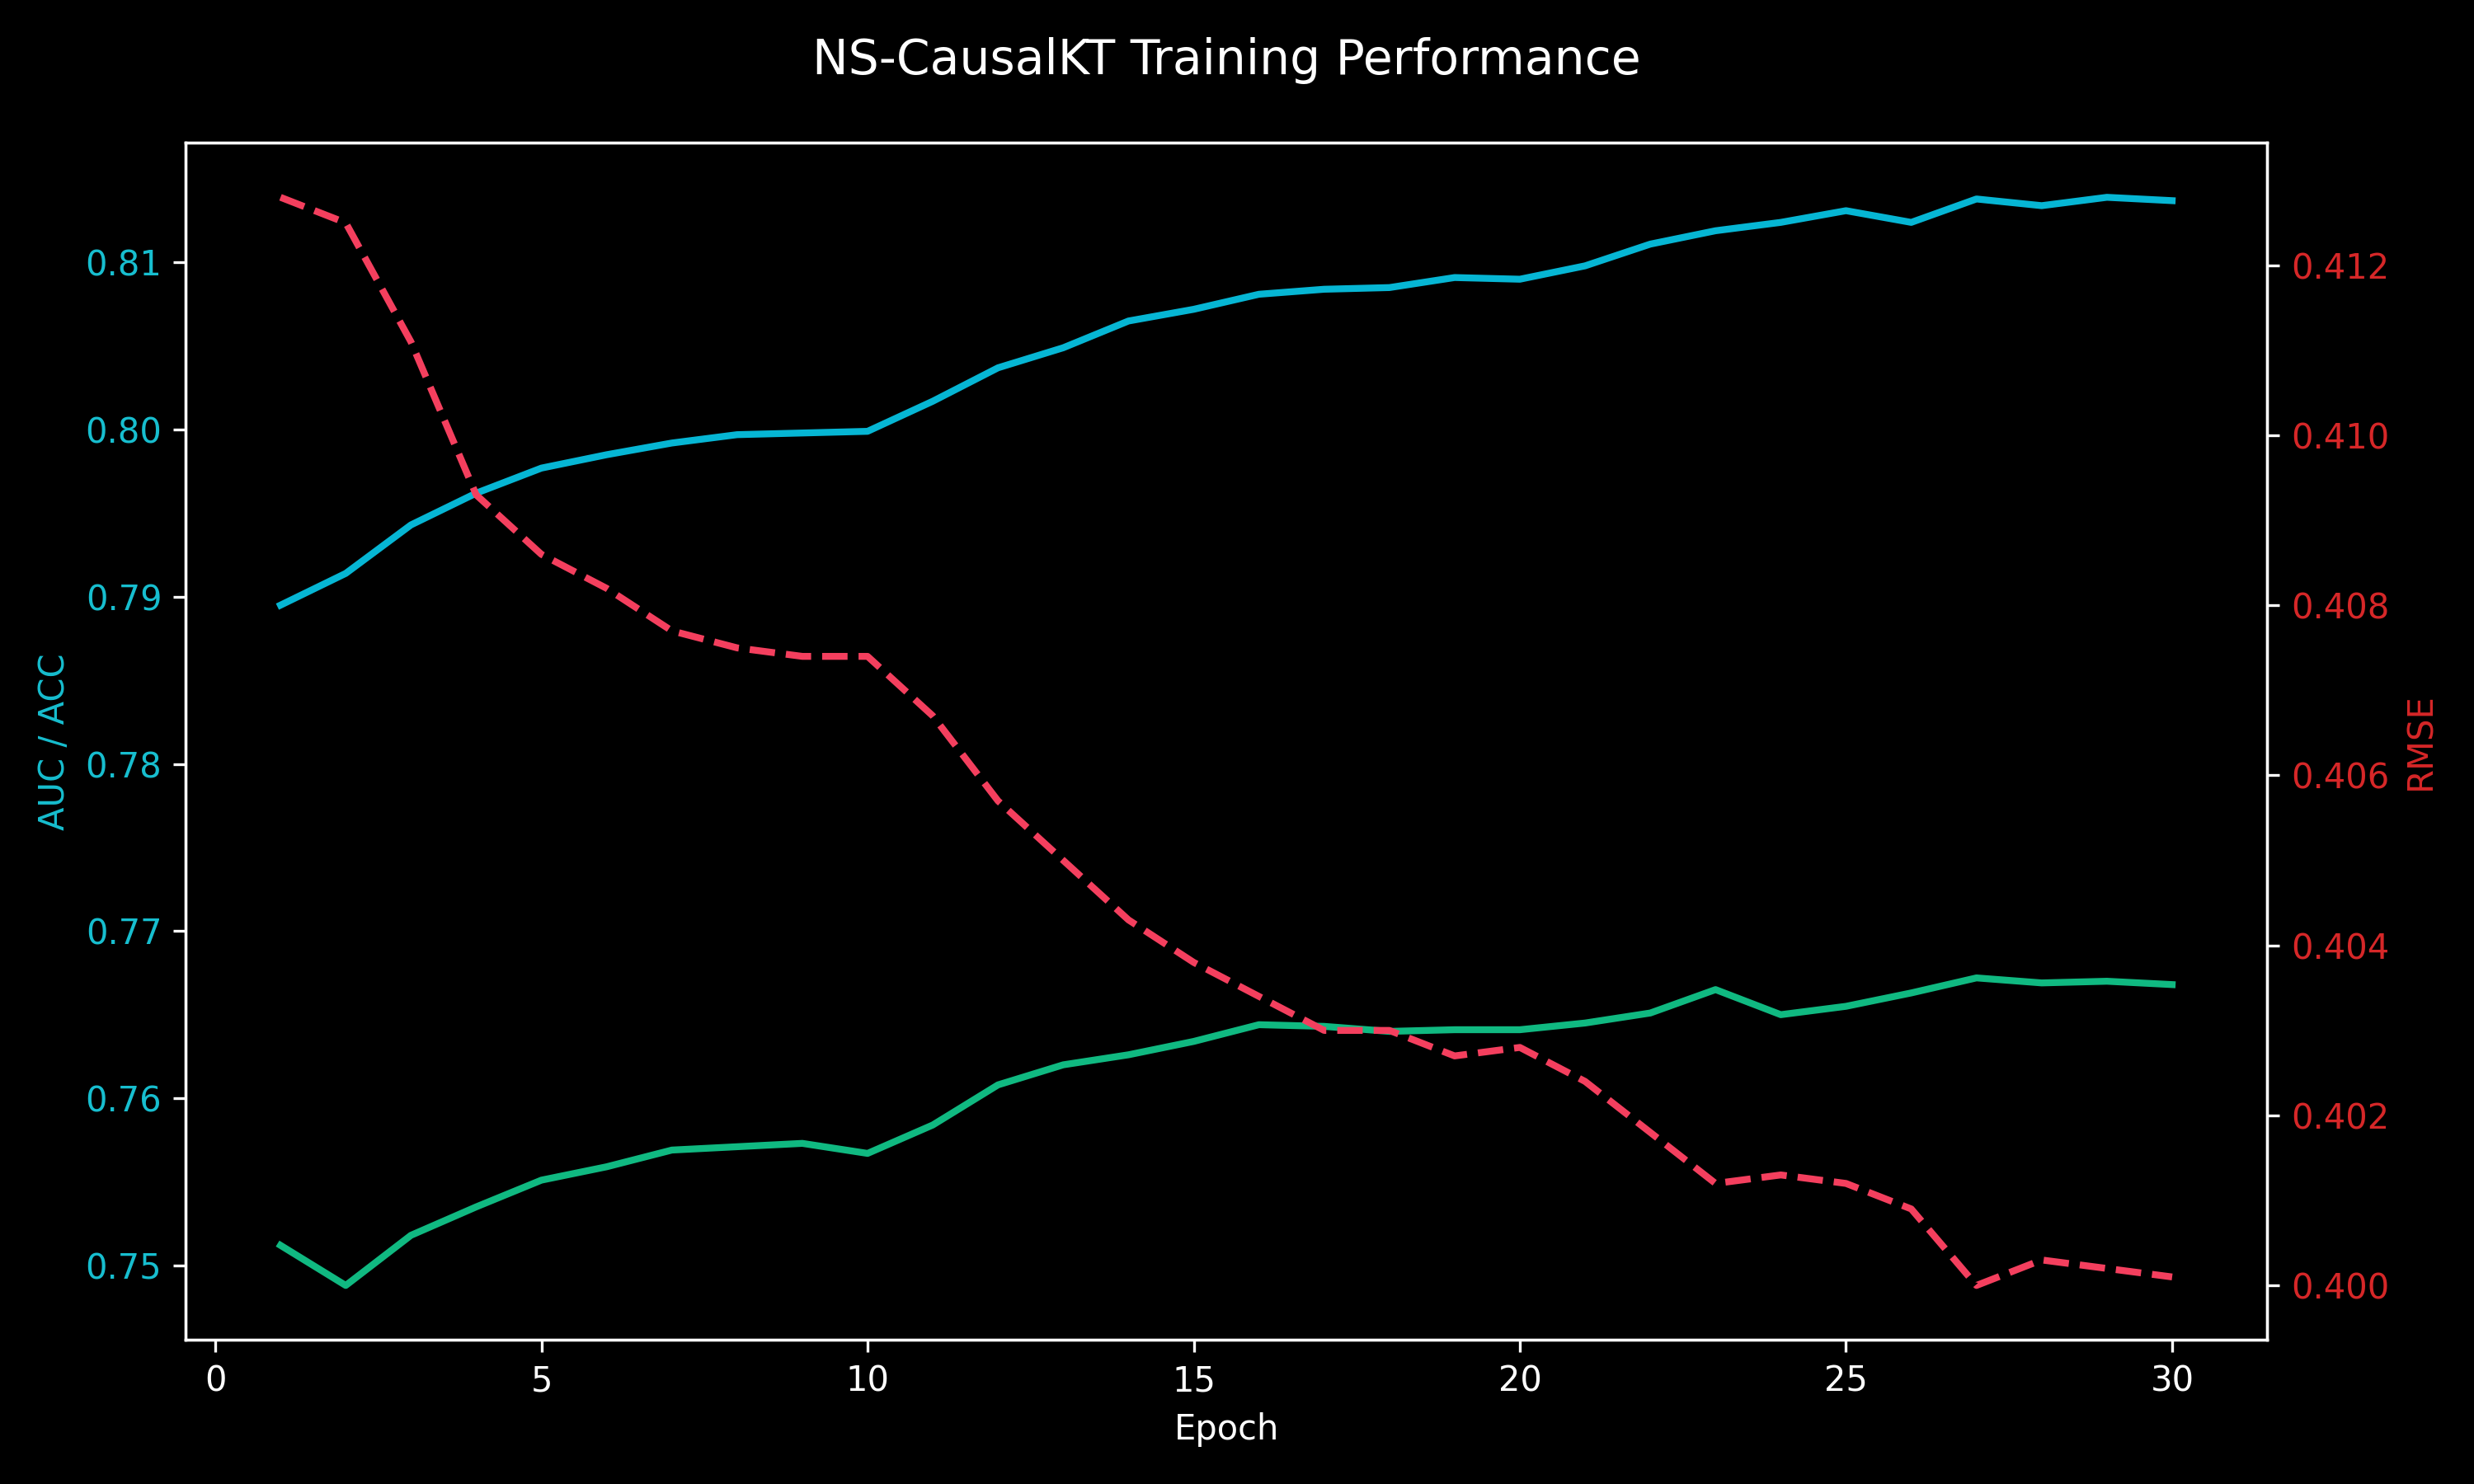
\includegraphics[width=\linewidth]{training_metrics.png}
    \caption{Training-curve artifact included in the repository report.}
    \label{fig:training}
\end{figure}

\section{Causal Visual Diagnostics}
The visualization folder contains student-level mastery heatmaps and counterfactual intervention plots. Fig.~\ref{fig:heatmaps} shows example heatmaps for two students, while Fig.~\ref{fig:counterfactuals} shows corresponding counterfactual bars. These views are designed for mentor-facing diagnosis: heatmaps reveal where mastery is unstable, and intervention plots summarize which concept changes are expected to affect success probability.

\begin{figure*}[t]
    \centering
    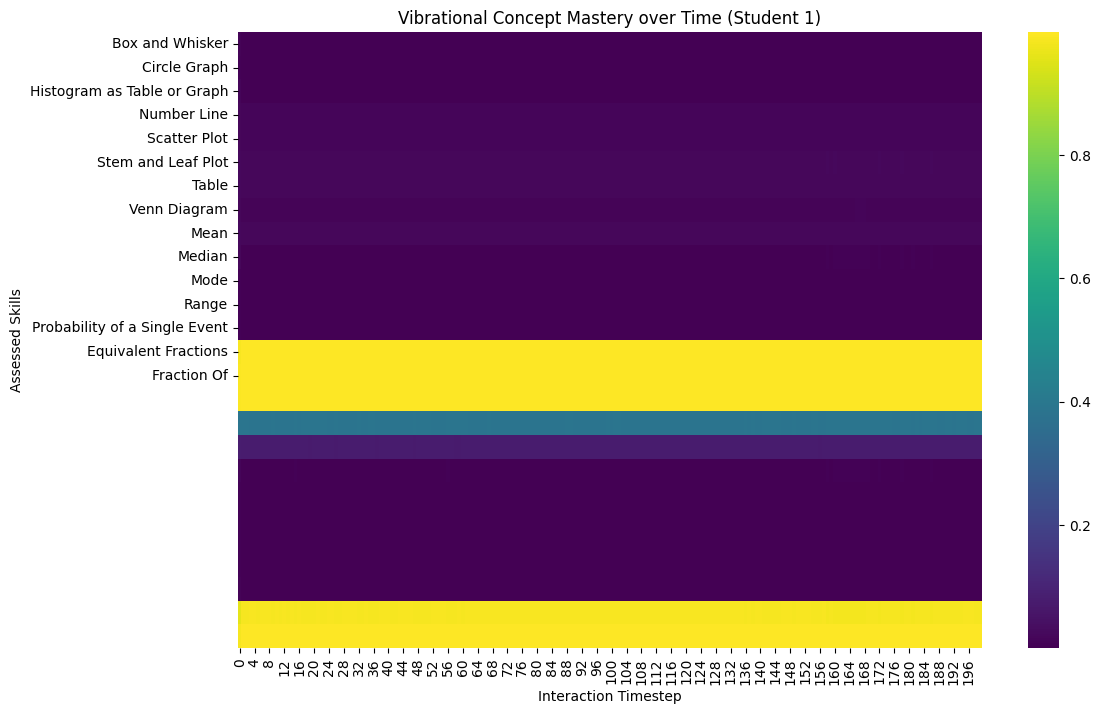
\includegraphics[width=0.48\textwidth]{student_1_heatmap.png}
    \hfill
    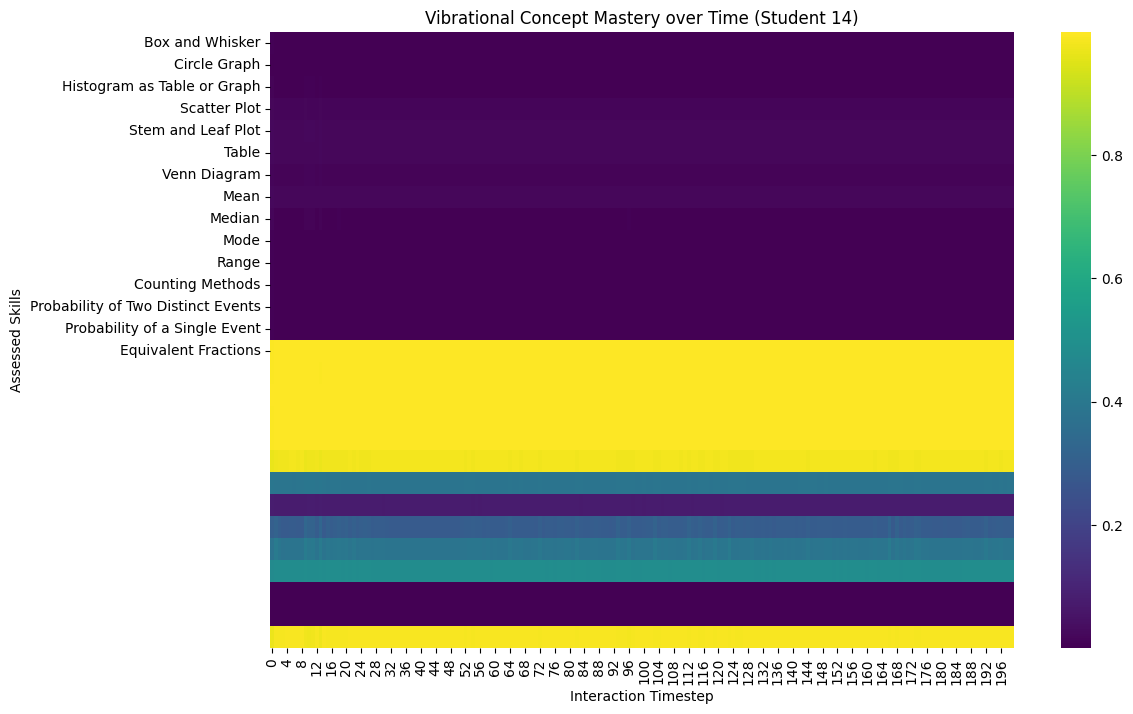
\includegraphics[width=0.48\textwidth]{student_14_heatmap.png}
    \caption{Student-level concept mastery heatmaps generated by the visualization pipeline.}
    \label{fig:heatmaps}
\end{figure*}

\begin{figure*}[t]
    \centering
    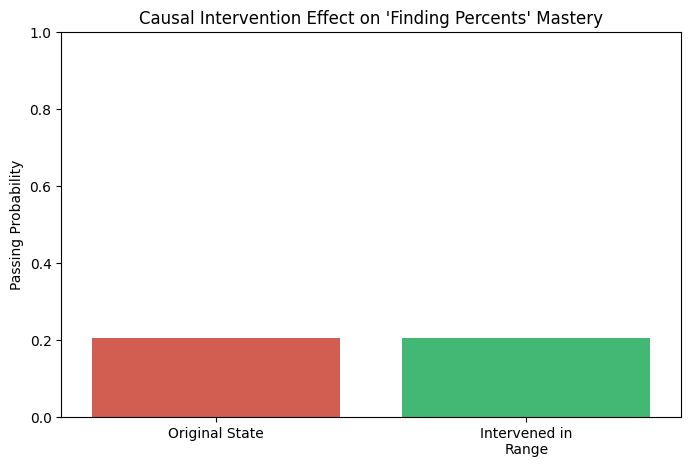
\includegraphics[width=0.48\textwidth]{student_1_counterfactual.png}
    \hfill
    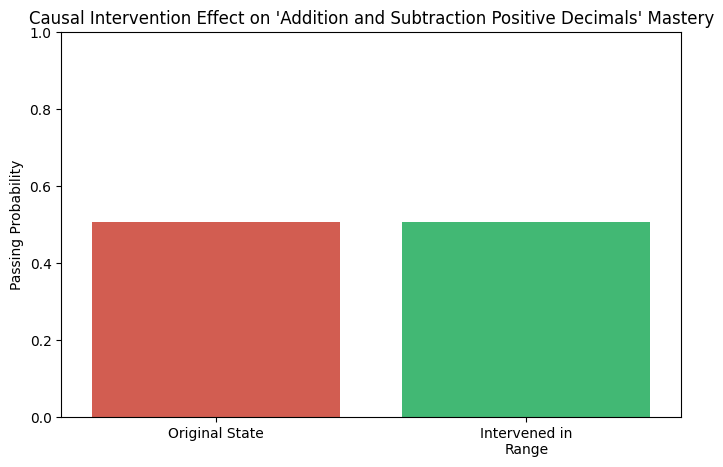
\includegraphics[width=0.48\textwidth]{student_14_counterfactual.png}
    \caption{Counterfactual intervention visualizations for selected students.}
    \label{fig:counterfactuals}
\end{figure*}

\subsection{Interpreting Heatmaps}
The heatmaps are intended to be read longitudinally. A stable high-mastery band suggests that a learner can reliably use the concept across time. A sudden drop suggests either forgetting, a shift to harder items, or noisy observations. A persistent low-mastery band suggests a candidate prerequisite gap. In practice, a mentor would combine this view with the student's recent work, curriculum position, and counterfactual ranking.

\subsection{Interpreting Counterfactual Bars}
The counterfactual bars summarize intervention sensitivity. If increasing mastery of a prerequisite concept yields a large predicted improvement on a target concept, the dashboard can recommend that prerequisite for remediation. If all bars are small, the model may be uncertain, the target item may depend on an unmodeled skill, or the student's failure may be due to non-concept factors such as attention or reading comprehension. This makes the visualization useful not only for recommending actions but also for exposing uncertainty.

\section{Ablation and Extension Plan}
The repository is already structured in separable model modules, which makes ablation straightforward. A publication-ready study should evaluate the following variants:
\begin{table}[t]
\centering
\caption{Recommended ablation study for the next experimental pass.}
\label{tab:ablation}
\begin{tabular}{p{0.37\linewidth}p{0.51\linewidth}}
\toprule
Variant & Purpose \\
\midrule
NSM only & Measures the neural backbone without symbolic or causal regularization. \\
NSM + SCL & Tests whether prerequisite consistency improves calibration and diagnostics. \\
NSM + CSL & Tests intervention diagnostics without symbolic graph correction. \\
Full NS-CausalKT & Measures the combined architecture. \\
Random graph & Checks whether graph structure matters or only regularization helps. \\
Validated graph & Measures improvement from curriculum-quality prerequisite edges. \\
\bottomrule
\end{tabular}
\end{table}

In addition to AUC and RMSE, ablations should report rule-satisfaction scores, intervention consistency, and root-cause agreement on synthetic planted-gap learners. These metrics are essential because the main claim is not merely that NS-CausalKT predicts correctness; it is that it exposes a more useful representation for educational intervention.

\section{Case Study Workflow}
Consider a learner whose next target item is tagged as quadratic equations. The model first estimates the probability of correctness and the current mastery vector. The dashboard then traces ancestors of the target concept in the prerequisite graph, such as arithmetic, fractions, algebraic manipulation, and linear equations. For each candidate prerequisite, the causal diagnostic layer clamps mastery, propagates the intervention through the graph, and recomputes predicted success. The largest positive effect is surfaced as the likely root-cause concept.

This workflow produces a teacher-facing explanation of the form: the student is predicted to struggle with the target item, and the largest expected improvement comes from remediating a specific prerequisite. The explanation can be checked against the student's answer sheet. For example, a sign error while rearranging an equation may support a recommendation to revisit linear equation manipulation before assigning additional quadratic practice. This is the central user experience goal of NS-CausalKT: to connect model output with a concrete next teaching action.

\section{Threats to Validity}
\subsection{Internal Validity}
The largest internal threat is graph validity. If prerequisite edges are wrong, symbolic correction can enforce misleading relationships and causal interventions can recommend the wrong concept. Another threat is the approximate nature of the current causal layer. Mastery clamping is useful for simulation, but it does not by itself prove causal identification. The system should therefore be described as intervention-oriented and causal-inspired unless validated against stronger causal evidence.

\subsection{External Validity}
ASSISTments 2009 is a widely used benchmark, but it represents a specific platform, subject distribution, and historical student population. Results may not transfer directly to other curricula, languages, age groups, or assessment styles. The agentic grading interface also depends on the quality of answer artifacts; handwritten work, scanned PDFs, and typed answers may require different preprocessing.

\subsection{Construct Validity}
Correctness is an imperfect proxy for mastery. A student may guess correctly, make a careless mistake, or know a concept but misunderstand an item statement. Response time is also ambiguous: long time can indicate effort, confusion, or distraction. NS-CausalKT partially addresses this by combining temporal history, concept graph structure, and answer artifacts, but the model still depends on noisy educational measurements.

\section{Ethical and Privacy Considerations}
Educational AI systems can affect student opportunity, teacher judgment, and learner confidence. A causal explanation that appears authoritative may be over-trusted, especially when presented in a polished dashboard. For this reason, NS-CausalKT should be deployed as decision support rather than automated judgment. The system should show evidence, uncertainty, and the relevant concept history, while leaving final instructional decisions to educators.

Privacy is equally important. Student interaction histories and answer sheets can contain sensitive information. The local KT pipeline is a strength because it can run without exposing raw records to hosted services. If multimodal grading is used, deployments should minimize uploaded data, redact personally identifying information, and provide a local model option for sensitive settings. Logs and stored uploads should be governed by clear retention policies.

\section{Future Work}
The immediate next step is to replace the surrogate prerequisite graph with a validated concept dependency graph. This could be built from curriculum standards, teacher annotations, platform metadata, or graph-mining methods followed by human review. The second step is to implement full ablations and matched baselines. The third step is to evaluate explanations with teachers: do ACE-ranked recommendations match expert judgment, and do they lead to better remediation choices?

Additional extensions include cold-start evaluation, zero-shot concept transfer, and richer causal variables such as hint usage, attempt count, question difficulty, and session context. A stronger SCM could explicitly model latent ability, item difficulty, and time effects. Finally, the agentic grading module can be improved by replacing hosted multimodal calls with a local document-understanding model for privacy-sensitive deployments.

\section{Discussion}
The prototype demonstrates a practical path for making KT outputs more explainable and actionable. The symbolic layer encodes curriculum structure, which helps translate latent probabilities into concept-level statements. The causal layer makes intervention simulation a first-class interface element, so the dashboard can answer questions such as which prerequisite should be remediated first.

The current implementation also exposes limitations. First, the prerequisite graph used during training is a surrogate sequential graph when a validated curriculum ontology is unavailable. Second, the causal layer approximates intervention effects through mastery clamping and graph propagation rather than a fully identified SCM with explicit confounder adjustment. Third, benchmark parity requires controlled training budgets, repeated seeds, and consistent splits. Finally, agentic grading must be evaluated carefully under privacy constraints and may require a local vision model for sensitive student work.

\section{Conclusion}
NS-CausalKT is a neural-symbolic causal KT prototype that shifts educational modeling from opaque score prediction toward explainable intervention planning. The current system trains successfully on ASSISTments 2009, produces usable mastery and counterfactual visualizations, and integrates with a deployable dashboard. Future work should replace the surrogate prerequisite graph with validated curriculum graphs, implement stronger causal identification tests, reproduce baselines under matched settings, and evaluate teacher-facing explanations with human users.

\section*{Acknowledgment}
This draft was prepared from the repository documentation, source files, training logs, benchmark logs, and visualization artifacts in the NS-CausalKT-Agentic-Grader project.

\bibliographystyle{IEEEtran}
\bibliography{references}

\end{document}
